\chapter{相关知识背景}
%\section{密码分析学概述}
%\subsection{密码分析学的发展背景}
%在古代,人类就已经开始使用密码用于保护外交和军事通信,而随着科技和信息技术的发展,在当今互联网性信息时代,大量的敏感和机密信息,如网上银行账户、私人信件、各个账户的密码等,都是常通过非可信的互联网来进行传输和交换的,然而对于这些信息的机密性、完整性和可用性是人们迫切需要的。因此,随之而来的信息安全问题日益突出,信息的安全威胁主要来自黑客攻击、计算机病毒、拒绝服务、中间人攻击、嗅探重放等。这就需要一个安全可靠的系统来保护信息的安全,目前人们对信息安全越来越重视,因此也有越来越多的人从事密码分析的研究。
%\subsection{密码分析学的定义}
%密码分析学是一门研究在不知道通常解密所需要的秘密信息的情况下对加密信息进行解密的学科,是密码学的一个分支,它的主要目的是研究信息的破解和信息的伪造。试图发现明文或密钥的过程就叫做密码分析。密码分析人员使用的策略取决于加密方案的特性和分析人员可用的信息。密码分析学是对密码算法进行分析或破译,在未知密钥的情况下,从密文推出明文或密钥的技术。密码编码学和密码分析学这两门学科尽管表面上看来是相互对立,但在整个密码学的发展过程中,却又是相辅相成、相互促进的。

%在一个不可信的信息传输和处理系统中,除了合法的接收者外,还有非授权者,他们通过窃听、中间人攻击和重发攻击等手段来获取机密信息。他们虽然不知道系统所用的密钥,但通过分析可能从截获的密文分析出原来的明文甚至加密算法的密钥,这一过程称作密码分析\cite{feng01}。从事这一工作的人称作密码分析员或密码分析者。一个密码是可破的,是指的通过密文能够在可容忍代价下分析出明文或密钥,或者通过明文一密文对能够确定密钥。
%\subsection{密码分析学研究的必要性}
%虽然密码分析的目标在密码学的历史上从古至今都一样,实际使用的方法和技巧则随着密码学变得越来越复杂而日新月异。密码学算法和协议从古代只利用纸笔等工具,发展到第二次世界大战时的恩尼格玛密码机,直到目前的基于电子计算机的方案。而密码分析也随之改变了。无限制地成功破解密码已经不再可能。事实上,只有很少的攻击是实际可行的。在上个世纪70年代中期,公钥密码学作为一个新兴的密码学分支发展起来了。而用来破解这些公钥系统的方法则和以住完全不同,通常需要解决精心构造出来的纯数学问题。其中最著名的就是大数的质因数分解。

%对密码进行分析主要是为了发现加密算法、密钥或密码系统的弱点,以完善加密过程,更有利于信息的安全。另一方面,是为了掌握密码分析者或破译者攻击密码的方法,找出其方法的漏洞,便于预防他们的攻击。同时也是为了更进一步提高广大计算机用户的安全意识和知识水平,减少针对系统的非法入侵和攻击带来的损失。因此,进行密码分析是非常必要的。
\section{密码分析方法}
\label{sec:2.4}
密码学在\cite{feng02}中可以分为经典密码学和现代密码学,而我们现在研究分析的主要领域在现代密码学,现代密码学包括分组密码算法、消息摘要算法、非对称密钥算法、公/私钥签名算法等。
密码分析可以从不同的角度进行分类,并且每种方法之间也没有严格的界限,在这里我们根据上述密码学中密码体制的类型来对密码分析方法进行大体分类。密码分析方法从大的方面可分为:古典密码分析方法,对称密码分析方法,非对称密码分析方法。因为密码有序列密码和分组密码之分,所以对称密码分析方法又分为序列密码分析方法和分组密码分析方法。现有的大多数非对称密码都属于分组密码,所以对非对称密码分析方法不再从这方面分类。本文主要讨论的是针对密码算法中密钥分析的很实用的一些方法,如穷举法、查表法、时空折中法。
\subsection{密码攻击类型}
我们在进行密码分析时是在假设密码分析者知道目标体统所使用的加密体制和密码算法的前提下进行的,也就是密码分析者可以根据密码算法得到明文和密文等方面的信息。这样我们可分将密码攻击为以下几种主要类型:
\begin{enumerate}
\item 唯密文攻击:密码分析者已知加密算法和待破译密文或部分密文,需要对信息加密的方法进行正确的猜测,对编码者的编码风格及密文的题材有一定的了解。
\item 己知明文攻击:密码分析者已知加密算法,有一些明文及相应的密文。用这些信息推出用于产生密文的信息。
\item 选择明文攻击:也称差分密码分析。密码分析者有机会使用密码机,且己知加密算法、待破译的密文、由密码分析者选择的明文信息。密码分析者用一个密钥对他所选择的明文加密以获得结果中的密文,但密钥本身不能被分析,密码分析者通过将整个密文与最初的明文作比较推出密钥。
\item 选择密文攻击:密码分析者已知加密算法,待破译的密文和密码分析者选择的猜测性密文。密码分析者将自己猜测的密文发给信息的实际接收者,接收者解密后得到一些杂乱的数据,于是他可能将这些杂乱的数据寄回给信息发送者或者以不安全的方式存储,则密码分析者可通过某些手段可能得到这些杂乱数据,再与猜测的密文作比较可推出密钥。
\item 选择文本:密码分析者已知加密算法,待破译的密文,密码分析者选择的明文信息及其对应的由密钥生成的密文,密码分析者选择的猜测性密文及其对应的由密钥生成的已破译的明文。密码分析者通过他所掌握的这些所有信息可推出密钥。
\end{enumerate}
上述是密码攻击的主要五种类型。这五种攻击类型的强度按序递增,唯密文攻击是最弱的一种攻击,最容易防护,因为密码分析者拥有的可供利用信息量最少。选择密文和选择文本是最强的攻击,如果一个密码系统能够抵抗这两个攻击,那么它当然能够抵抗其余三种攻击,这两者很少被使用,但他们也是可能的攻击
途径。对一个密码系统采取截获密文进行分析的这类攻击称作被动攻击。

密码系统还可能遭受到的另一类攻击是主动攻击,非法入侵者主动向系统采用监听、删除、修改、增添、重放、伪造等手段向系统注入假消息。防止这种攻击的一种有效方法是使发送的消息具有可被验证的能力,使接收者或第三者能够识别和确认消息的真伪,实现这类功能的密码系统称作认证系统。消息的认证性和消息的保密性不同,保密性是使截获者在不知道密钥的条件下不能解读密文的内容,而认证性是使任何不知道密钥的人不能构造出一个密报,使意定的接收者解密成为一个可理解的消息(合法的消息)。

进行密码分析时,我们还应考虑一种密码攻击的复杂度,当然复杂度越低越好。可将密码攻击复杂度分为两部分,数据复杂度和处理复杂度。数据复杂度是实施该攻击所需输入的数据量;而处理复杂度是处理这些数据所需的计算量。这两部分的主要部分通常被用来刻划该攻击的复杂度。例如,在穷举密钥搜索攻击中,所需要的数据量与计算量相比是微不足到的,因此,穷尽密钥搜索攻击的复杂度实际是处理复杂度。在差分密码分析中,实施攻击所需的计算量相对于所需的明密文对的数量来说是比较小的,因此,差分密码分析的复杂度实际是数据复杂度。
\subsection{暴力攻击法}
暴力攻击法可用于任何分组密码算法和消息摘要算法,而且攻击的复杂度只依赖于分组长度和密钥长度,暴力攻击主要有:穷举密钥攻击、字典攻
击、查表攻击、时间-存储攻击。

穷举密钥搜索攻击中,设k是密钥长度(以比特为单位),在唯密文攻击下,攻击者依次试用密钥空间中所有$2^k$个密钥解密一个或多个截获的密文,直至得到一个或多个有意义的明文块。在已知(选择)明文攻击下,攻击者试用密钥空间中的所有$2^k$个密钥对一个已知明文加密,将加密结果同该明文相对应的已知密文比较,直至二者相等,然后再用其他几个已知明密文对来验证该密钥的正确性。穷举密钥搜索的复杂度平均为$2^{k-1}$次加密,实际上这种攻击方法适用于任何密码体制。

字典攻击中,攻击者搜集明密文对,并把它们编排成一个“字典”。攻击者
看见密文时,检查这个密文是否在字典里,如果在,他就获得了该密文相对应的
明文。如果n是分组长度,那么字典攻击需要$2^n$个明密文对才能使攻击者在不
知道密钥的情况下加解密任何消息。

查表攻击中,设k是密钥长度,查表法采用选择明文攻击,其基本观点是:
对一个给定的明文x,用所有$2^k$个密钥K(记其全体为K),欲计算密文$y_k=E_k(x)$。构造一张有序对表${(y_k,K)}_{k\in K}$,以$y_k$给出K的标号。因此,对于给定的密文,攻击者只需从存储空间中找出相对应的密钥K即可。

时间-空间折中攻击法是一种选择明文攻击方法,它由穷尽密钥搜索攻击和查表攻击两种方法混合而成,它在选择明文攻击中以时间换取空间。它比穷尽密钥搜索攻击的时间复杂度小,比查表攻击的空间复杂度小。
如图\ref{fig:2.1}所示,比较了这种暴力攻击方法的特点:
\begin{figure}[!ht]
\centering
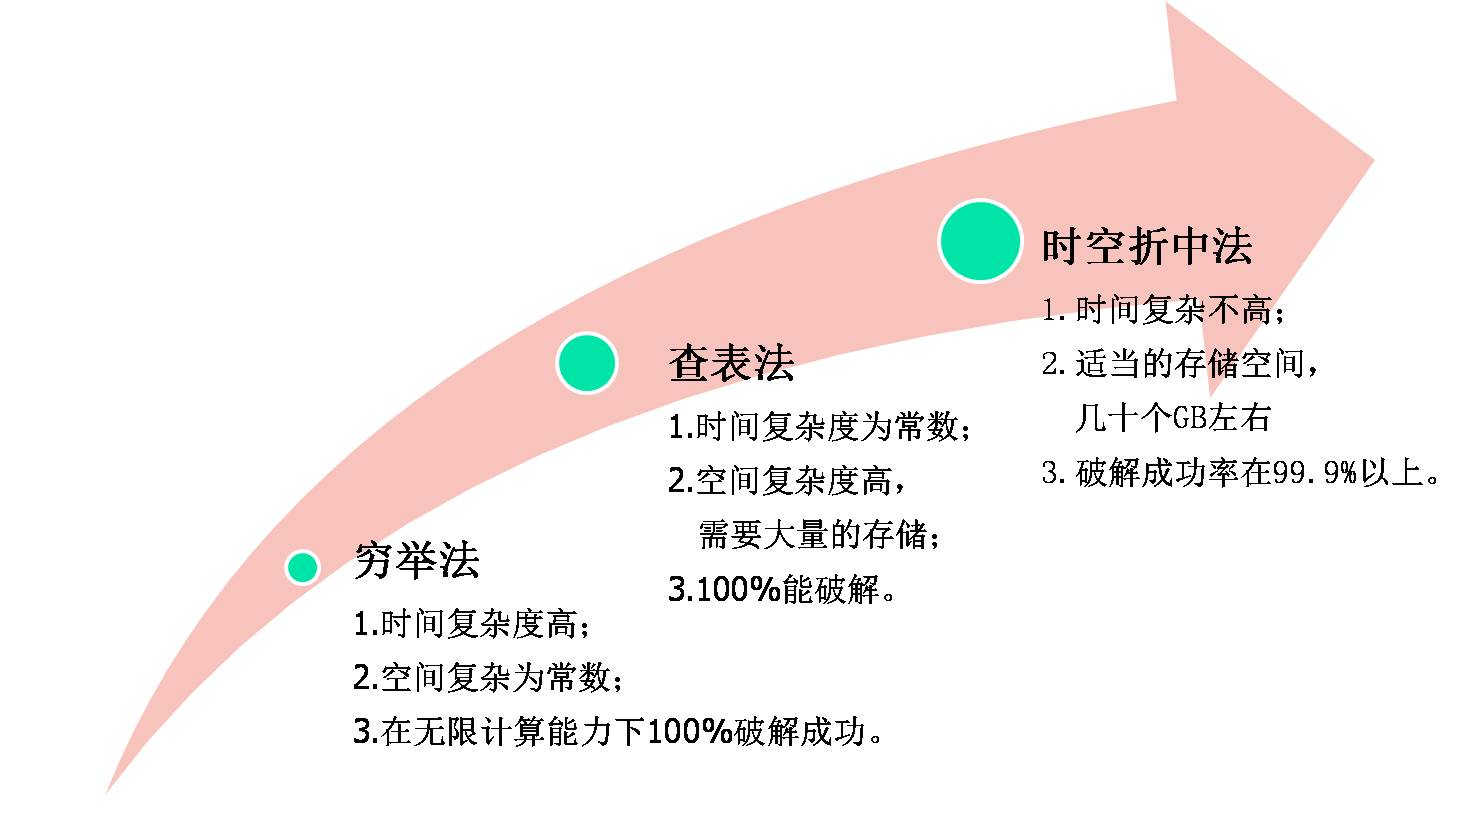
\includegraphics[scale=0.5]{2-1.jpg}
\caption{暴力攻击的几个方法比较}
\label{fig:2.1}
\end{figure}
\section{单向散列函数}
\subsection{Hash函数的简介}
单向散列函数,又称单向Hash函数、杂凑函数,就是把任意长的输入消息串变化成固定长度的输出串的一种不可逆函数。这个输出串称为消息的散列值。一般用于密钥加密,产生消息摘要等。单向散列函数是现代密码学的一个重要领域,它是数据完整性检测、数字签名和认证方案中必不可少的一部分。单向Hash函数\cite{hash}是许多协议框架中的一个模块。目前由许多Hash函数的公开算法,一般一个安全的Hash函数应该至少满足以下几个条件:
\begin{enumerate}
\item 输入串值的长度是任意的;
\item 输出串Hash值长度是固定的;
\item 对每个给定的输入串的值,计算机得到输出Hash值是很容易的;
\item 给定Hash函数的描述,已知一个Hash值时,要找到输入串使它的的Hash值等于已知的这个Hash值在计算上时不可行的,或是找到两个不同的输入串,计算得到相同的输出Hash值在计算上是不可行的。
\end{enumerate}
Hash函数主要用于数据完整性校验和数字签名的有效性,常被用在身份认证上。例如在一个身份验证系统上,保存用户的密码时,需要把密钥用Hash算法进行加密,得到一个Hash值。由于Hash函数本身的特点,其他用户即使得到了这个Hash值也无法还原密码。当用户登录时,系统把用户输入的密码再用Hash算法进行计算,得到的Hash值与保存在系统中的Hash值进行比较,从而验证用户的合法性。
MD5\cite{md5}(Message-Digest Algorithm 5)是目前应用最广泛的 Hash 函数之一。MD5 将任意长度的“字节串”变换成一个 128比特的大整数,并且它是一个不可逆的字符串变换算法,换句话说就是,即使你看到源程序和算法描述,也无法将一个 MD5 的值变换回原始的字符串,从数学原理上说,是因为原始的字符串有无穷多个,这有点象不存在逆函数的数学函数。MD5在经过一些初始处理后,将明文分成了512位的块,再将每一块分成16个32位的子块。算法的输出是4个32位的块,连接起来就是128位的输出的Hash值。
\subsection{对Hash函数攻击的方法}
\begin{enumerate}
\item 替换法

这是一个十分实用的攻击方法,它并不对Hash算法本身作任何攻击,只是利用系统中的Hash函数重新生成一个Hash值,这个Hash值的输入串是攻击者已知的,如“password”,这样我们就可能把这串新生成的Hash值替换掉系统本身的Hash值,此时攻击者就能用“password”能登陆系统,从而达到绕过系统的认证机制。这种攻击方法需要攻击者已知目标系统认证机制使用的Hash算法函数(一般的系统都使用MD5算法函数)和由替换的权限。
\item 字典查表法

还有一种在实际破解中使用较多得方法是字典查询法,攻击者需要预先对目标Hash算法构造相应得字典文件,然后把需要破解得Hash值跟这个字典文件里得Hash值进行检索比较,通常这种办法需要TB级甚至跟大得存储空间,并且预运算的时间代价也是很大的。
\item 碰撞法

所谓杂凑碰撞指两个完全不同的讯息经杂凑函数计算得出完全相同的杂凑值。根据鸽巢原理,以有长度限制的杂凑函数计算没有长度限制的讯息是必然会有冲撞情况出现的。可是,一直以来,电脑保安专家都认为要任意制造出冲撞需时太长,在实际情况上不可能发生。2004年8月17日的美国加州圣巴巴拉的国际密码学会议(Crypto’2004)上,来自中国山东大学的王小云教授做了破译MD5、HAVAL-128、 MD4和RIPEMD算法的报告,公布了MD系列算法的破解结果。在破解MD5之后,2005年2月,王小云教授又破解了另一国际密码SHA-1,王小云的研究成果表明了从理论上讲电子签名可以伪造,必须及时添加限制条件,或者重新选用更为安全的密码标准,以保证电子商务的安全。2005年8月,王小云、姚期智,以及姚期智妻子姚储枫(即为Knuth起名高德纳的人)联手于国际密码讨论年会尾声部份提出SHA-1杂凑函数杂凑冲撞演算法的改良版。此改良版使破解SHA-1时间缩短。

曾与王小云共同攻破完整 MD5 算法的中科院的冯登国与长沙国防科大的谢涛最近在 IACR 上发布了一篇题为《仅用一个消息块实现 MD5 碰撞》的文章。出于安全因素的考虑,文章中并未公开具体实现方法,但他们向全球密码学爱好者发出挑战:第一个在 2013 年 1 月 1 日之前找出新的单块碰撞的人将获得一万美元的奖励。他们公布的产生碰撞的消息块为:
0x6165300e,0x87a79a55,0xf7c60bd0,0x34febd0b,0x6503cf04,0x854f709e,\\
0xfb0fc034,0x874c9c65,0x2f94cc40,0x15a12deb,0x5c15f4a3,0x490786bb,\\
0x6d658673,0xa4341f7d,0x8fd75920,0xefd18d5a\\
0x6165300e,0x87a79a55,0xf7c60bd0,0x34febd0b,0x6503cf04,0x854f749e,\\
0xfb0fc034,0x874c9c65,0x2f94cc40,0x15a12deb,0xdc15f4a3,0x490786bb,\\
0x6d658673,0xa4341f7d,0x8fd75920,0xefd18d5a\\
这两个消息块有两处不同,但 MD5 均为 0xf999c8c9 0xf7939ab6 0x84f3c481 0x1457cb23。
\end{enumerate}
\section{CUDA并行计算相关知识}
\subsection{GPU并行计算概述}
GPU即图形处理器,目前,主流计算机的处理器主要是中央处理器CPU和图形处理器GPU。传统上,GPU只负责图形渲染,而大部分的处理都交给了CPU。然而GPU在处理能力和存储器带宽上相对CPU有明显优势,在成本和功耗上也不需要付出太大代价。
2007年6月,NVIDIA公司推出了CUDA,CUDA不需要借助图形学API,而是采用了类C语言进行开发。同时,CUDA的GPU采用了统一处理架构,以及引入了片内共享存储器,这大大降低了基于GPU的并行计算程式的开发难度。CUDA为开发人员有效利用GPU的强大性能提供了条件。自推出后,CUDA被广泛应用于密码破解、石油勘测、天文计算、流体力学模拟、分子动力学仿真、生物计算、图像处理、音视频编解码的领域,在很多应用中获得了几倍、几十倍、甚至上百倍的加速比。

在现代计算机体系结构中属于显卡外设的一个专门图形处理器。随着人们对显卡并行性的研究和开发,我们对它的可编程性也提出了更高的需求。比如从Nvidia Geforce 8系列的显卡开始,英伟达公司就在其上面配置了大量的可独立运行计算的处理器核心。在2010年的ISCA大会上,英特尔公司向大会递交了一份关于GPU和CPU的测试技术文档,在文档中正式承认GPU的运行速度比CPU快14倍\cite{intel}。测试中英特尔采用的是GeForce GTX 280,在当时是英伟达上一代产品,并且没有经过任何代码优化,而实际上新一代的NVIDIA GPU的运行速度是英特尔CPU的上百倍。
\begin{figure}[!ht]
\centering
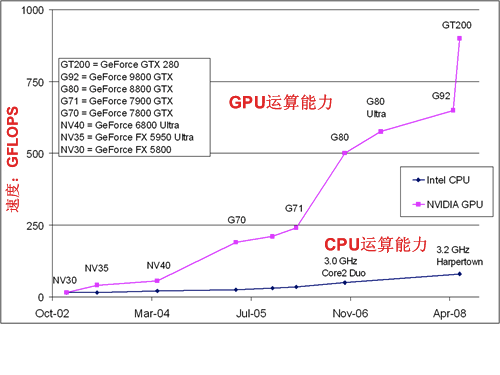
\includegraphics[scale=0.8]{cpu-gpu}
\caption{GPU和CPU速度对比}
\label{fig:2.1}
\end{figure}

英伟达公司通过对显卡增加一些硬件接口,使得对显卡的编程已经不再需要像操作硬件设备那样依赖特定的语言和程序接口。他们提出了CUDA的编程模型,这个编程模型是为了方面开发者能够便捷快速地在Nvida显卡上开发应用程序。
\subsection{CUDA体系结构}
2007年6月,NVIDIA公司推出了CUDA\cite{nvidia},它是一个开发应用程序的平台,或者说是一种编程模型。该模型将用户应用程序代码分为两部分:宿主(Host)代码和设备(Device)代码。宿主代码由CPU负责串并行化的处理,而设备代码则是交给一个或多个GPU并发处理。同时每个CUDA处理器都支持单指令多数据(SIMD)方法\cite{nb},可以使得所有核心处理器上并发运行的线程基于相同的代码。虽然由于数据的不同会导致产生分支,但是仍然支持全局的内存共享。下图\ref{fig:2.2}为Nvidia GeForce 8800显卡的工作示意图,我们可以看到程序从主存把数据拷贝到GPU的显存里,然后在GPU中每个核心处理器中进行并行计算,最后把结果拷贝回主存里。
\begin{figure}[!ht]
\centering
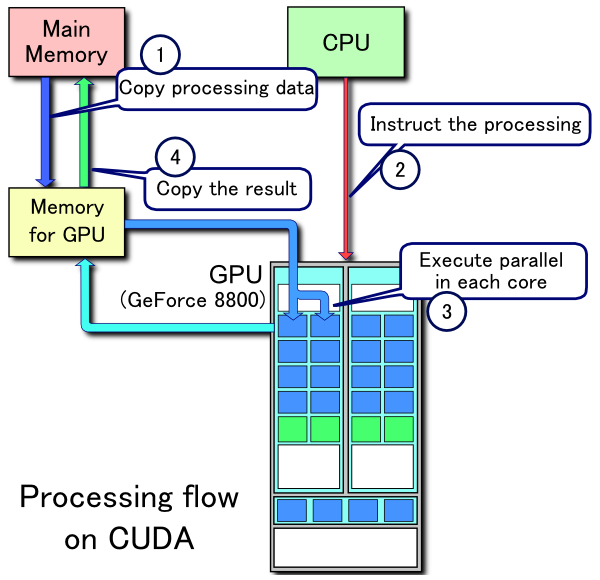
\includegraphics[scale=0.5]{cuda}
\caption{GPU并行运算体系结构}
\label{fig:2.2}
\end{figure}

CUDA程序由nvcc编译器执行,编译流程如图\ref{fig:2.3}所示。代码运行期间,程序执行可能循环经历宿主态和设备态的转换,这种转换其实质是CPU和GPU之间的转换,我们应该尽量减少这样的状态转换,避免上下文切换带来的代价。因此在编程阶段应当尽量使GPU能运行足够长的时间。
\begin{figure}[!ht]
\centering
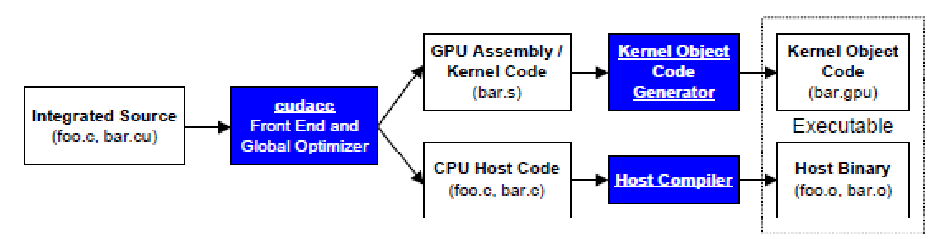
\includegraphics[scale=0.4]{2-3}
\caption{CUDA的编译流程}
\label{fig:2.3}
\end{figure}
\subsection{Fermi构架}
Fermi是NVIDIA公司最新一代的显卡构架代号,在2010年3月27日,NVIDIA公司正式发布Fermi构架的桌面显卡GeForce GTX480。Fermi是新一代CUDA计算与图形构架,针对双精度运算、ECC内存容错能力、Cache体系结构、上下文切换和原子读写操作等方面进行了全面的设计,通过新的构架设计不仅仅增加了计算能力,并且支持更好的可编程能力和计算效果。
Fermi构架有如下主要新的特性:
\begin{enumerate}
\item 第三代Streaming Multiprocessor(SM)
	\begin{itemize}
	\item 每个SM包含32个CUDA Core,是GST200的4倍 
	\item 8倍于GT200的双精度浮点性能
	\item Dual Warp调度策略,一个周期内可启动两个warp进行计算
	\item 每个SM有64KB的RAM,可灵活地配置共享内存和L1缓存
	\end{itemize}
\item 第二代PTX ISA架构(PTX 2.0)
	\begin{itemize}
	\item 统一寻址空间,完整支持C++特性
	\item 针对OpenCL和DirectCompute进行优化设计
	\item 完整支持IEEE 754-2008 32bit/64bit精度
	\item 通过Predication(断言)来提高性能
	\end{itemize}
\item 改进的内存操作子系统
	\begin{itemize}
	\item 可配置的L1和统一的L2并行数据高数缓存
	\item 内存支持ECC校验
	\item 极大增强原子内存操作性能
	\end{itemize}
\item 第三代千兆线程引擎(GigaThread 3.0)
	\begin{itemize}
	\item 比上一代强10倍的上下文切换能力
	\item 并发核心程序执行机制
	\end{itemize}
\end{enumerate}
%\section{XFS文件系统}
%\section{存储技术}
%这里我们主要介绍三种存储技术:DAS、NAS和SAN。
%\subsection{直接附加存储}
%直接附加存储方式与我们普通PC的存储构架一样,外部的存储设备都是直接连接在服务器的内部总线上,是整个服务器结构的一部分。

%DAS存储方式主要使用与以下环境:
%\begin{enumerate}
%\item 小型网络

%因为网络规模较小,数据存储量小,且也不是很复杂,采用这种存储方式对服务器的影响不会很大。并且这种存储方式也十分经济,适合拥有小型网络的企业用户。
%\item 地理位置分散的网络

%虽然企业总体网络规模较大,但在地理分布上很分散,通过SAN或NAS在它们之间进行互联非常困难,此时各分支机构的服务器也可采用DAS存储方式,这样可以降低成本。
%\item 特殊应用服务器

%在一些特殊应用服务器上,如微软的集群服务器或某些数据库使用的原始分区,均要求存储设备直接连接到应用服务器。
%\end{enumerate}
%\subsection{网络附加存储}
%NAS(网络附加存储)方式则全面改进了以前低效的DAS存储方式。它采用独立于服务器,单独为网络数据存储而开发的一种文件服务器来连接所存储设备,自形成一个网络。这样数据存储就不再是服务器的附属,而是作为独立网络节点而存在于网络之中,可由所有的网络用户共享。

%NAS的优点:
%\begin{enumerate}
%\item 真正的即插即用\quad NAS是独立的存储节点存在于网络之中,与用户的操作系统平台无关,真正的即插即用。
%\item 存储部署简单\quad NAS不依赖通用的操作系统,而是采用一个面向用户设计的,专门用于数据存储的简化操作系统,内置了与网络连接所需要的协议,因此使整个系统的管理和设置较为简单。
%\item 存储设备位置非常灵活 
%\item 管理容易且成本低\quad NAS数据存储方式是基于现有的企业Ethernet而设计的,按照TCP/IP协议进行通信,以文件的I/O方式进行数据传输。

%NAS的缺点:(1)存储性能较低 (2)可靠度不高
%\end{enumerate}
%\subsection{SAN存储方式}
%1991年,IBM公司在S/390服务器中推出了ESCON(Enterprise System Connection)技术。它是基于光纤介质,最大传输速率达17MB/s的服务器访问存储器的一种连接方式。在此基础上,进一步推出了功能更强的ESCON Director(FC SWitch),构建了一套最原始的SAN系统。

%SAN存储方式创造了存储的网络化。存储网络化顺应了计算机服务器体系结构网络化的趋势。SAN的支撑技术是光纤通道(FC Fiber Channel)技术。它是ANSI为网络和通道I/O接口建立的一个标准集成。FC技术支持HIPPI、IPI、SCSI、IP、ATM等多种高级协议,其最大特性是将网络和设备的通信协议与传输物理介质隔离开,这样多种协议可在同一个物理连接上同时传送。

%SAN的硬件基础设施是光纤通道,用光纤通道构建的SAN由以下三个部分组成:
%\begin{enumerate}
%\item 存储和备份设备:包括磁带、磁盘和光盘库等。
%\item 光纤通道网络连接部件:包括主机总线适配卡、驱动程序、光缆、集线器、交换机、光纤通道和SCSI间的桥接器
%\item 应用和管理软件:包括备份软件、存储资源管理软件和存储设备管理软件。
%\end{enumerate}

%SAN的优势:
%\begin{enumerate}
%\item 网络部署容易;
%\item 高速存储性能。因为SAN采用了光纤通道技术,所以它具有更高的存储带宽,存储性能明显提高。SAn的光纤通道使用全双工串行通信原理传输数据,传输速率高达1062.5Mb/s。
%\item 良好的扩展能力。由于SAN采用了网络结构,扩展能力更强。光纤接口提供了10公里的连接距离,这使得实现物理上分离,不在本地机房的存储变得非常容易。
%\end{enumerate}
%\subsection{DAS、NAS和SAN三种存储方式比较}
%存储应用最大的特点是没有标准的体系结构,这三种存储方式共存,互相补充,已经很好满足目前企业信息化应用。
%从连接方式上对比,DAS采用了存储设备直接连接应用服务器,具有一定的灵活性和限制性;NAS通过网络(TCP/IP,ATM,FDDI)技术连接存储设备和应用服务器,存储设备位置灵活,随着万兆网的出现,传输速率有了很大的提高;SAN则是通过光纤通道(Fibre Channel)技术连接存储设备和应用服务器,具有很好的传输速率和扩展性能。三种存储方式各有优势,相互共存,占到了现在磁盘存储市场的70\%以上。
\section{本章小结}
本章简要介绍了本文涉及到的相关知识背景,阐述了现代密码分析的方法手段和密码攻击的类型,比较了暴力攻击法的几种方法,穷举法的虽然可以100\%破解成功,但这是建立在付出巨大的计算代价和时间代价;查表法则以巨大的存储代价来达到密码破解的目的;而时空折中法则是前两种办法的折中办法,以空间代价换取时间代价或者以时间代价换取空间代价,在两个中间找到一个平衡点,这样会损失一些破解成功率。最后以单向散列函数的破解为例,介绍了对Hash函数加密了的密钥的破解。
介绍CUDA并行计算的相关知识,包括GPU并行计算体系结构以及CUDA编程模型,一个基本的CUDA程序由宿主程序和设备程序组成。
%最后介绍了三种存储方式技术:DAS、NAS和SAN。
